% imports and packages and stuff
% add or remove these as necessary
\documentclass[12pt]{article}
\usepackage[english]{babel}
\usepackage[utf8]{inputenc}
\usepackage{amsmath}
\usepackage{graphicx}
\usepackage{hyperref}
\usepackage{tabularx}
\usepackage[shortlabels]{enumitem}
\usepackage[parfill]{parskip}
\usepackage[letterpaper, portrait, margin=1in]{geometry}
\usepackage{color}


% % bibliography package
% \usepackage{csquotes}
% \usepackage[style=ieee]{biblatex}
% \addbibresource{references.bib}



% appendix package
\usepackage[title, titletoc]{appendix}

% font
\usepackage{palatino}

% make urls styled not weirdly
\urlstyle{same}

% change the spacing of tables to be reasonable
\renewcommand{\arraystretch}{1.5}

% start of the document
\begin{document}
\begin{titlepage}
\newcommand{\HRule}{\rule{\linewidth}{0.1mm}} 
\center % Center everything on the page
 
%---------------------------------------------------------------------------------
%	HEADING SECTION
%---------------------------------------------------------------------------------
\textsc{\Large ECE 445}\\[0.5cm] % heading course Number
\textsc{\large Senior Design Project}\\[0.5cm] % heading course name
\textsc{\Large Project Proposal }\\[0.5cm] % Minor heading
%---------------------------------------------------------------------------------
%	TITLE SECTION
%---------------------------------------------------------------------------------

\HRule \\[0.5cm]
\huge \textbf{Desktop-sized Environment-controlled Greenhouse for the Cultivation of multiple-type plants} % Title
\HRule \\[2cm]
 
%---------------------------------------------------------------------------------
%	AUTHOR SECTION
%---------------------------------------------------------------------------------
\begin{minipage}{0.5\textwidth}
    \begin{center} \large
        \underline{\textbf{Team \#2}} \\ \medskip
        \textsc{Zhimin Wang} (zhiminw2@illinois.edu) \\
        \textsc{Ze Yang} (zeyang2@illinois.edu) \\
        \textsc{Taoran Li} (taoranl2@illinois.edu) \\
        \textsc{Haoyu Qiu} (haoyuq2@illinois.edu)% Names and netID
    \end{center}
\end{minipage} \\[1.5cm]

\begin{minipage}{0.5\textwidth}
    \begin{center}
        \large
        \underline{TA}: Qi Wang
    \end{center}
\end{minipage} \\[1cm]

\begin{minipage}{0.5\textwidth}
    \begin{center}
        \large
        \underline{Sponsor}: Professor Wee-Liat Ong
    \end{center}
\end{minipage} \\[1cm]


{\large March 6, 2023} % Date

\vfill % Fill the rest of the page with white-space

\end{titlepage}
\pagenumbering{roman}
\setcounter{page}{2}
% \section*{Abstract} % * makes it so that the section is not numbered

 % include abstract in abstract.tex
% \clearpage
\tableofcontents
% \listoffigures % putting these here in case we need them later
% \listoftables
\newpage

% Below starts all the sections in their own individual files in the sections folder
\pagenumbering{arabic}

\clearpage
\section{Introduction}
A greenhouse (also called a glasshouse) is a structure with walls and a roof made chiefly of transparent material, such as glass, in which plants requiring regulated climatic conditions are grown.\cite{greenhouse}These structures range in size from small sheds to industrial-sized buildings, according to various objects. Although greenhouse technology has shown its value in different uses, a blank still exists in the field of a home ornamental greenhouse product for ordinary consumers, especially for those people who lived in a department in an urban area. There are still several obstacles and gaps that remain to be solved for such kinds of products.

% \subsection{Background}
\subsection{Background and Problem}
Greenhouse production plays a significant role in modern agriculture, especially in densely populated areas such as eastern China. Greenhouse environmental conditions have proven efficient and essential for crop yield, pest prevention, energy saving, etc.\cite{LI2020105096} As a productive system, the large-scale and medium-scale greenhouses allows us to respond to the growing global demand for fresh and healthy crops throughout the year, which is widely applied in agricultural production.\cite{rizwan2022optimal} Traditionally, small-scale greenhouses are used in agricultural experiments. Researchers cultivate their plants in a modular environment-controlled greenhouse, to gather data on the state of crop growth in a highly specified and optimized environment.

However, in most cases, traditional greenhouses are not intended for ordinary consumers. Even those greenhouse products marked for home use, are mainly for those customers who live in houses with gardens. It is not likely for a user who lived in a department to enjoy a greenhouse to plant for ornamental use. In fact, several obstacles remain to be solved for a customer greenhouse product. First, traditional greenhouse products are usually too large in their size. The most common glasshouse size for growers is 8 to 10 feet wide, however large greenhouses for sale may range from 12 to 20 feet in width.\cite{hartley_botanic} The greenhouse industry’s current practices can require considerable energy to power electric lighting to maintain plant growth on overcast days.\cite{watson_boudreau_van_iersel_2018} Excessive energy consumption also makes it not applicable for household use. Second, considering the above two factors, it is very inconvenient for the customers to install and carry away. The main cause for the large size and the high energy consumption is that the greenhouse environment is not easily controlled.\cite{rizwan2022optimal} As its climate parameters are interrelated, a specific amount of sensors should be installed in a comparably small model, which is the third problem. The last obstacle is that customers nowadays are more likely to be accustomed to using their phones to control devices in their homes.\cite{scott_2018} Currently, no full-featured app can adapt very well to product use in the market. There is still much room for improvement in this area.


% \subsection{Problems}
% \textcolor{blue}{below need to be modified}

\subsection{Overview of the Solution}
To solve the problems mentioned above, we plan to design a desktop-size environment-controlled greenhouse that can be used for ordinary customers. To reduce its size and energy consumption, only the necessary components would be kept in the product. The product is a cube space with an environment-controlling system. All the control functions will be implemented through the app on the mobile phone. The whole product's size is strictly controlled to be desktop-level. The energy consumption should be limited to about the same as general household appliances. 

\subsection{Visual Aid}
As shown in Fig. \ref{fig:visual_overview}, the whole model consists of three parts: a main growing space product with a water tank and a control board, a cloud server, and a mobile phone. The graphic design for the top and bottom levels of the model is shown in Fig. \ref{fig:visual_up} and Fig. \ref{fig:visual_low}.
\begin{figure}[!htb]
\centering
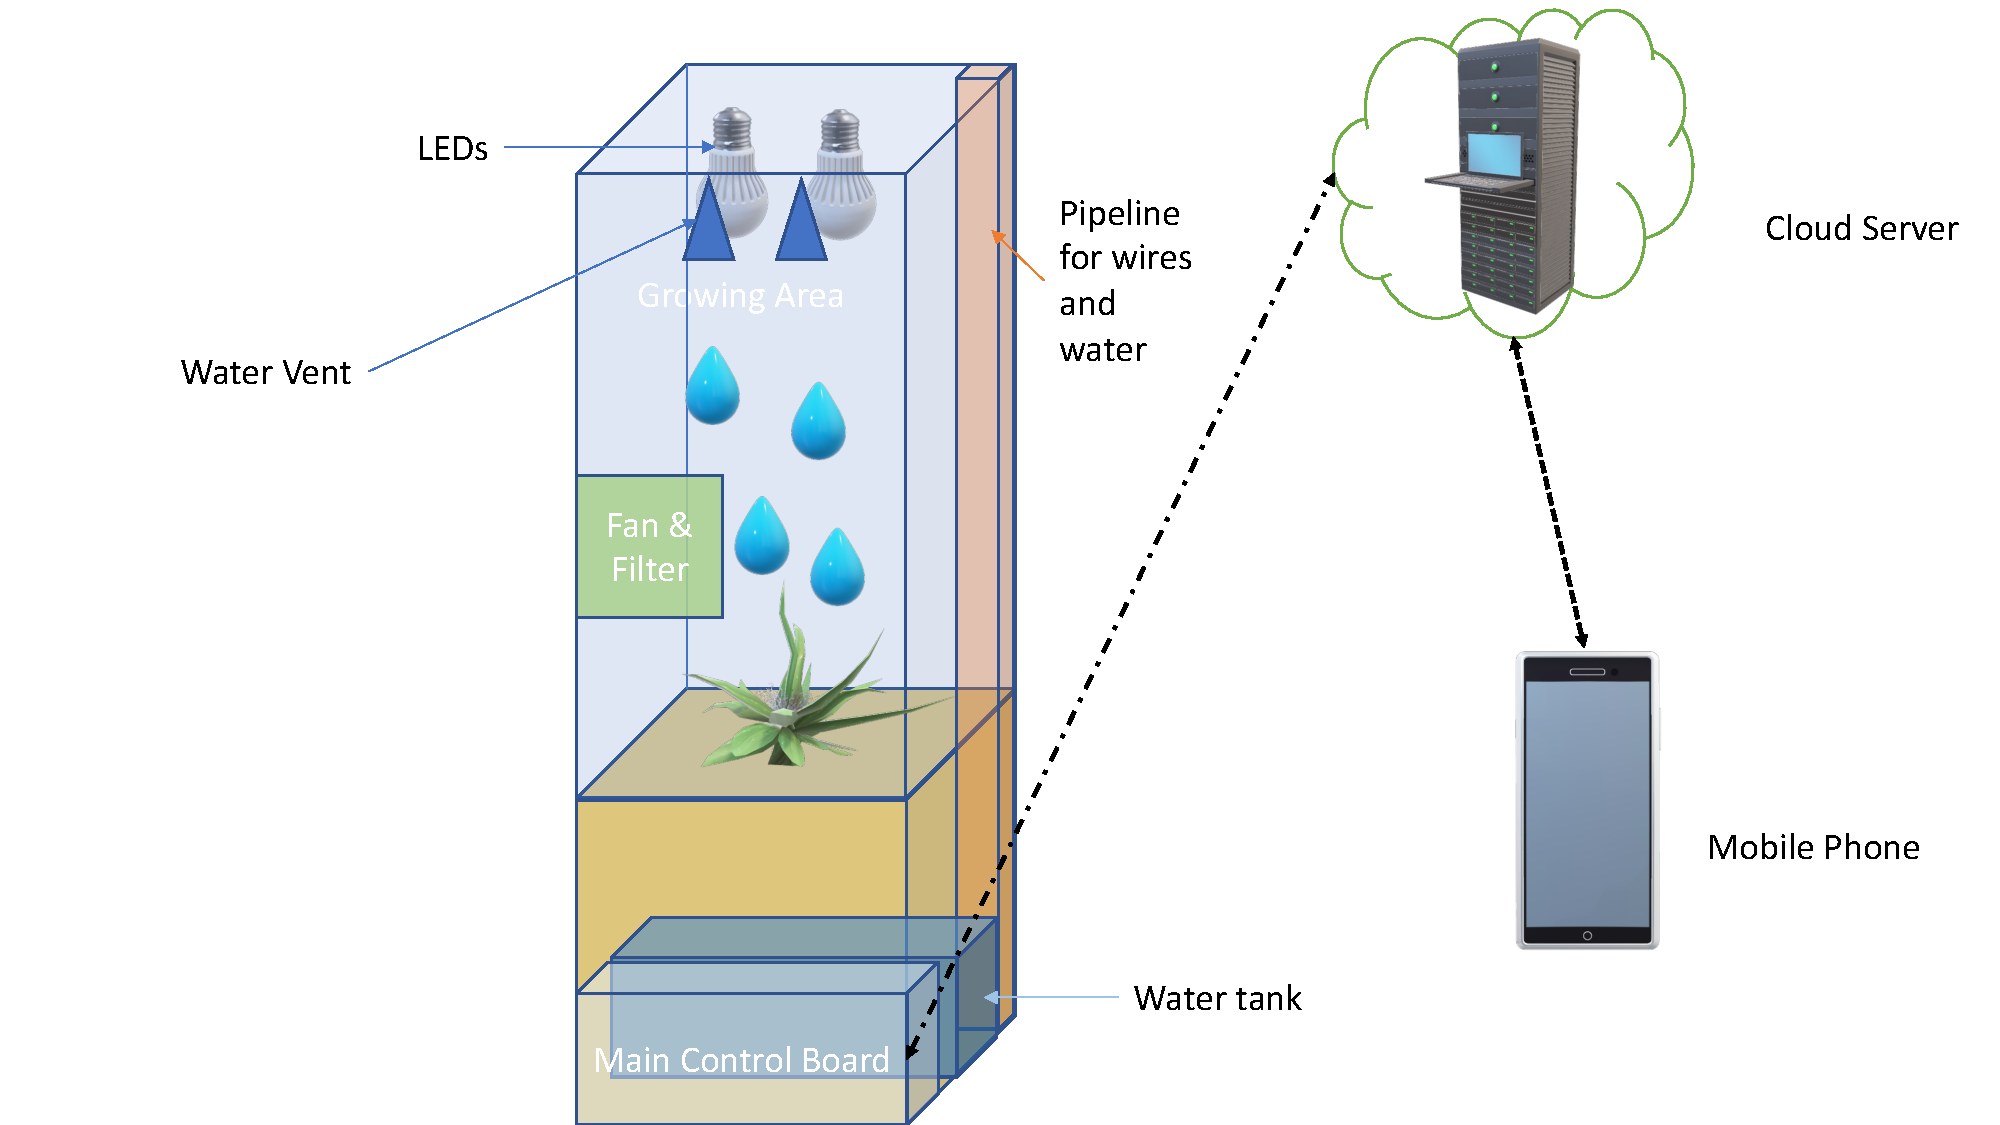
\includegraphics[width=0.8\textwidth]{Figure/visual_overview.pdf}
\caption{Overview of the model}
\label{fig:visual_overview}
\end{figure}

\begin{figure}[!htb]
\centering
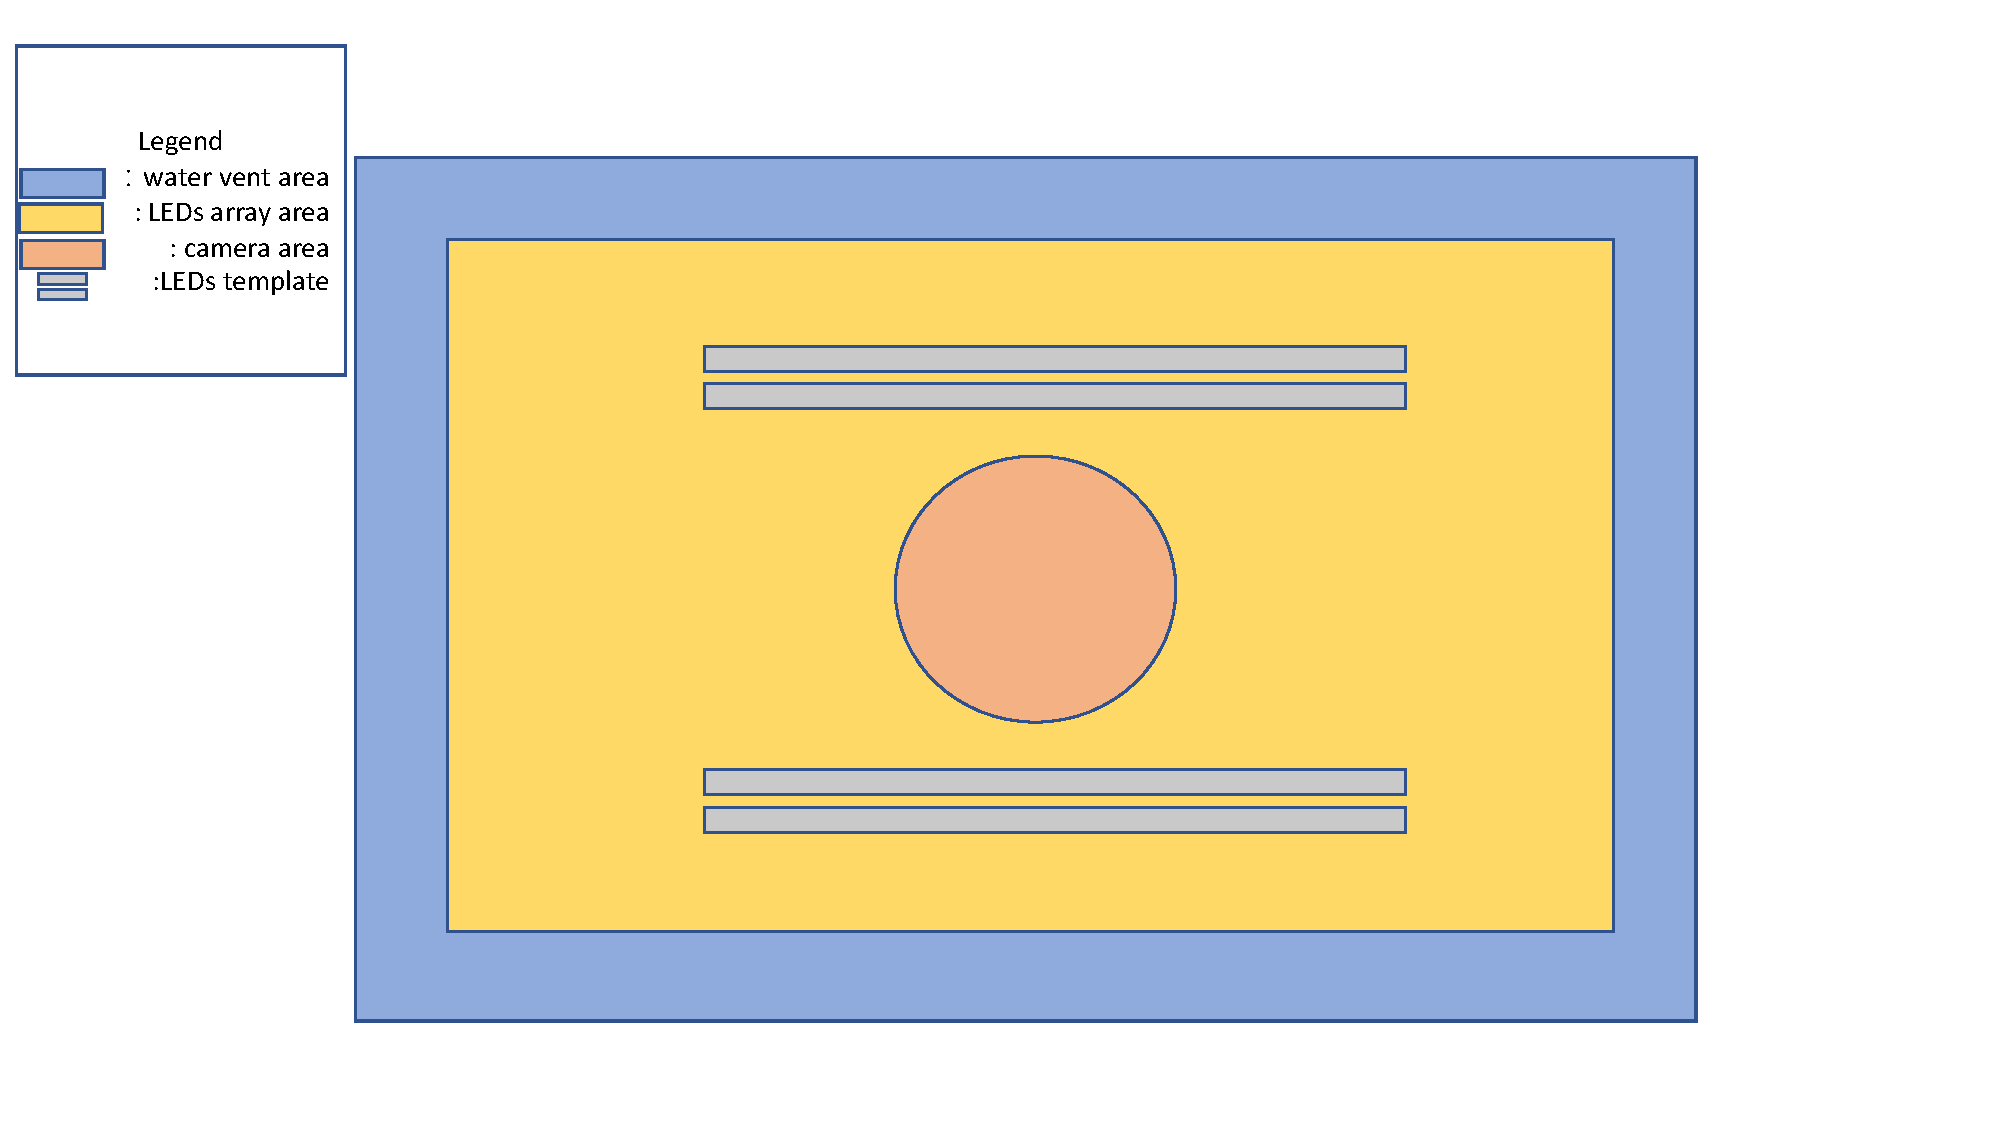
\includegraphics[width=0.8\textwidth]{Figure/upper_level.pdf}
\caption{Model's top platform design}
\label{fig:visual_up}
\end{figure}

\begin{figure}[!htb]
\centering
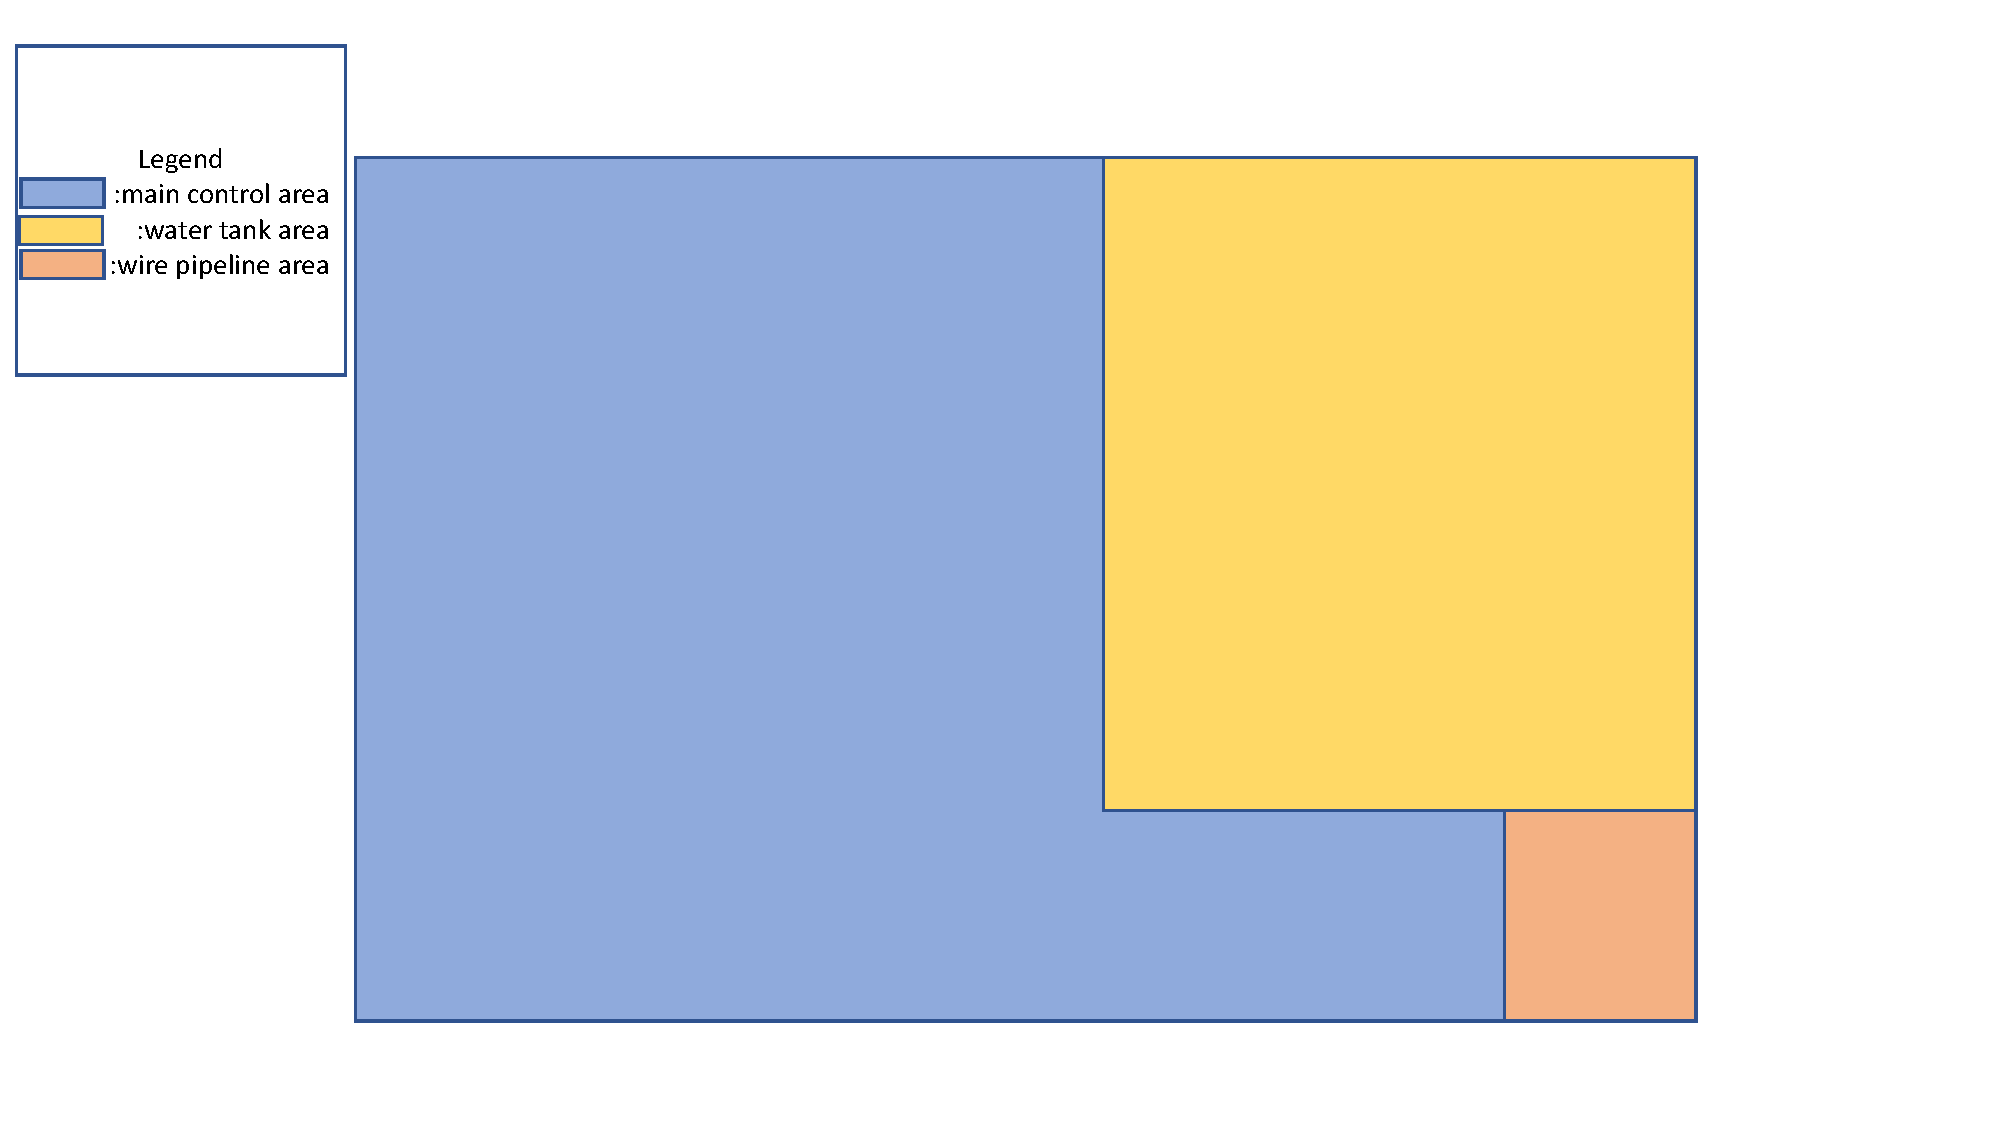
\includegraphics[width=0.8\textwidth]{Figure/lower_level.pdf}
\caption{Model's lower platform design}
\label{fig:visual_low}
\end{figure}

\clearpage

% A pictorial representation of your project that puts your solution in context. Include other external systems relevant to your project (e.g. if your solution connects to a phone via Bluetooth, draw a dotted line between your device and the phone). Note that this is not a block diagram and should explain how the solution is used, not a breakdown of inner components.

\subsection{High-Level Requirement List}
 % A list of three quantitative characteristics that this project must exhibit in order to solve the problem. Each high-level requirement must be stated in complete sentences and displayed as a bulleted list. Avoid mentioning "cost" as a high level requirement.
\begin{enumerate}
    \item There is a main planting cube. The model should be able to hold a fully functional environment-controlling system.
    \item The environment-controlling system includes:
        \begin{enumerate}
        \item Multiple adjustable LEDs to provide demanded light.
        \item A temperature-controlling system that can maintain the temperature.
        \item A humidity-controlling system that can maintain the humidity.
        \end{enumerate}
    \item A filter for the input and out gas, which should filter the harmful particles.
    \item A fan can input and output the air according to the demands.
    \item A camera that can monitor the plants: OV2640/OV5640 (have not determined)
    \item A 5V relay for the water vent.
    \item Several environment detectors should be installed, including:
        \begin{enumerate}
            \item Temperature: DHT22\cite{dht22}
            \item Humidity: DHT22\cite{dht22}
            \item Illumination detector.
            \item Air quality.
        \end{enumerate}
    \item A mobile phone app that can receive the data and adjust the settings.
\end{enumerate}
 % Copy the above 3 lines to add another section

\clearpage

\clearpage
\section{Design and Requirement}
\subsection{Block Diagram} 
The design's block diagram overview is shown in Fig. \ref{fig:overview_block_diagram}. In order to decrease the size of the accessories in the model, leaving more space for the growing area, only the necessary sensors and a chip microcontroller would be left in the model. The information collected by the sensors will be packaged and sent to a cloud server. The server will then process these data, sending them to the mobile phone. The users can view this information directly on their mobile phones, and adjust the environmental settings.

\begin{figure}[!htb]
\centering
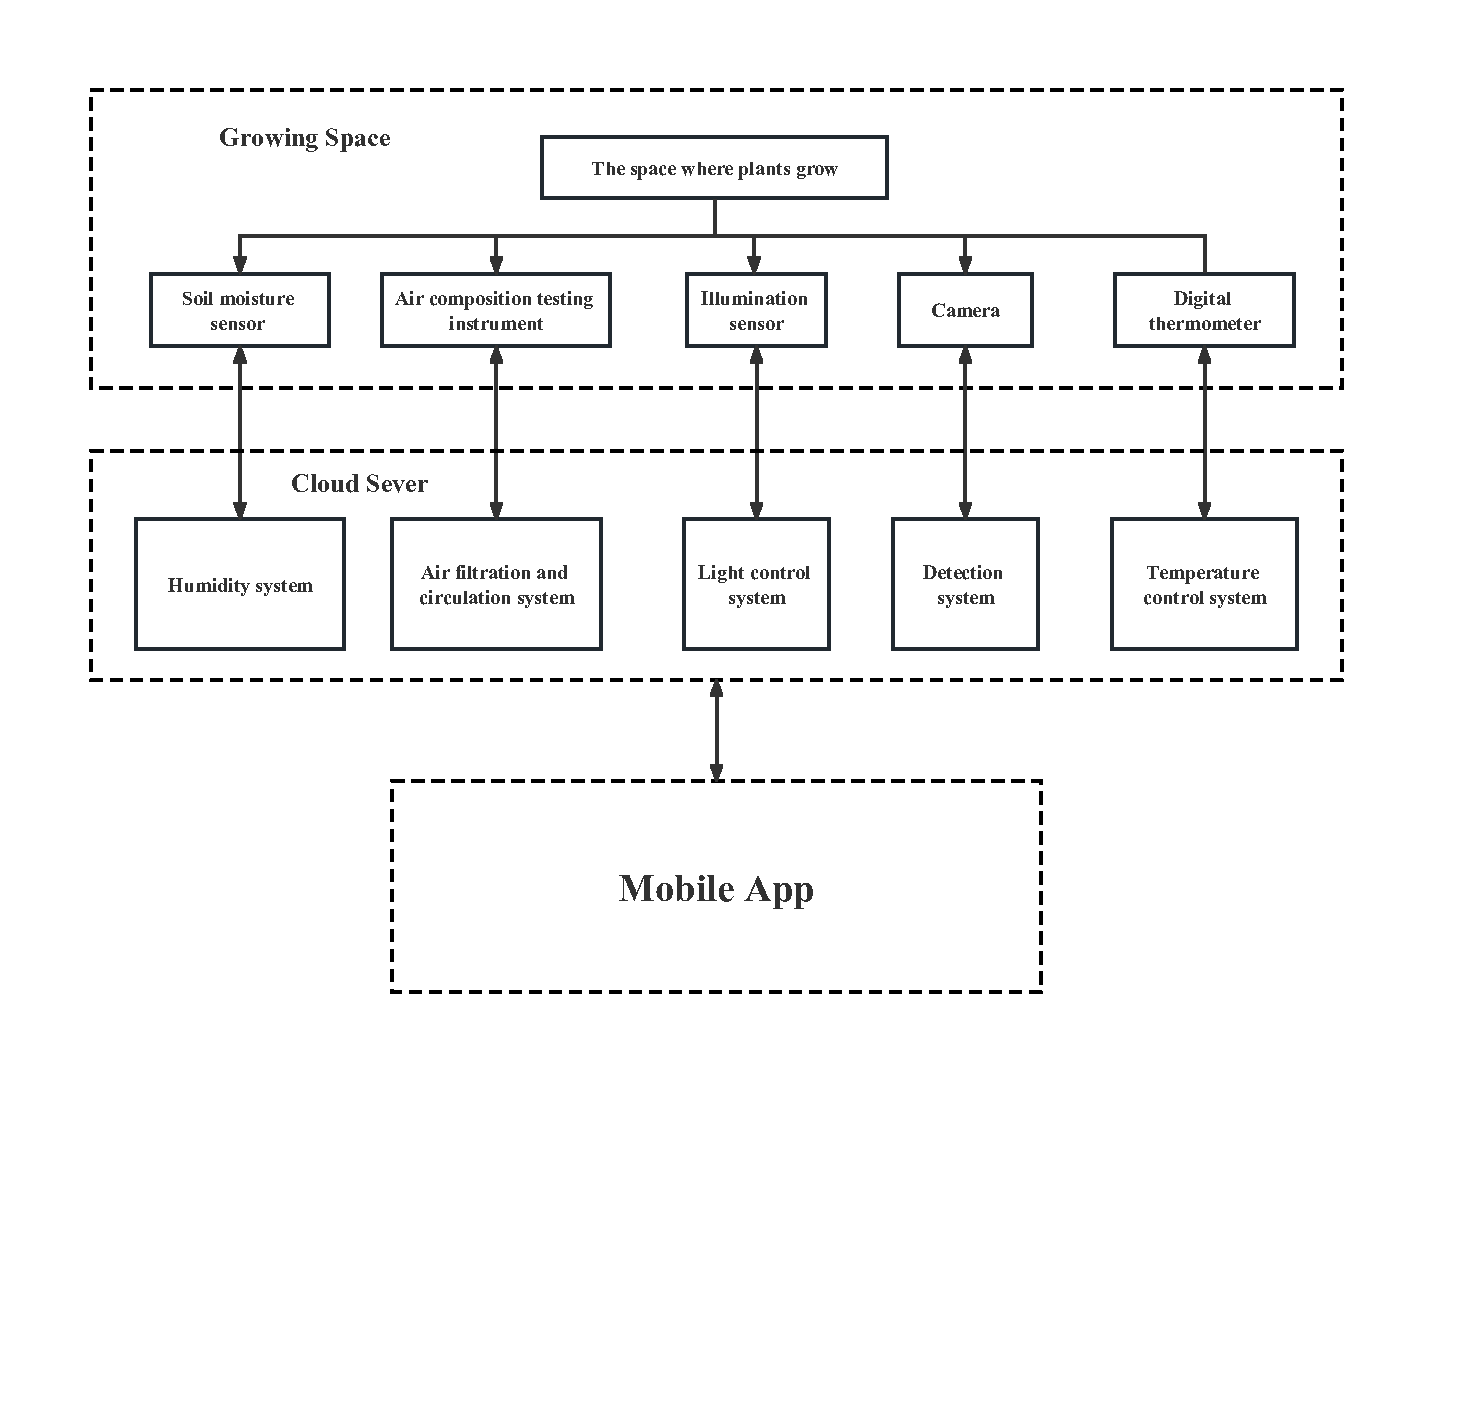
\includegraphics[width=0.8\textwidth]{Figure/block_overview.pdf}
\caption{Overview of block diagram}
\label{fig:overview_block_diagram}
\end{figure}


\subsection{Subsystem Overview} 
The detailed information of each block (subsystem) is shown in Fig. \ref{fig:d_block}. 

\begin{figure}[!htb]
\centering
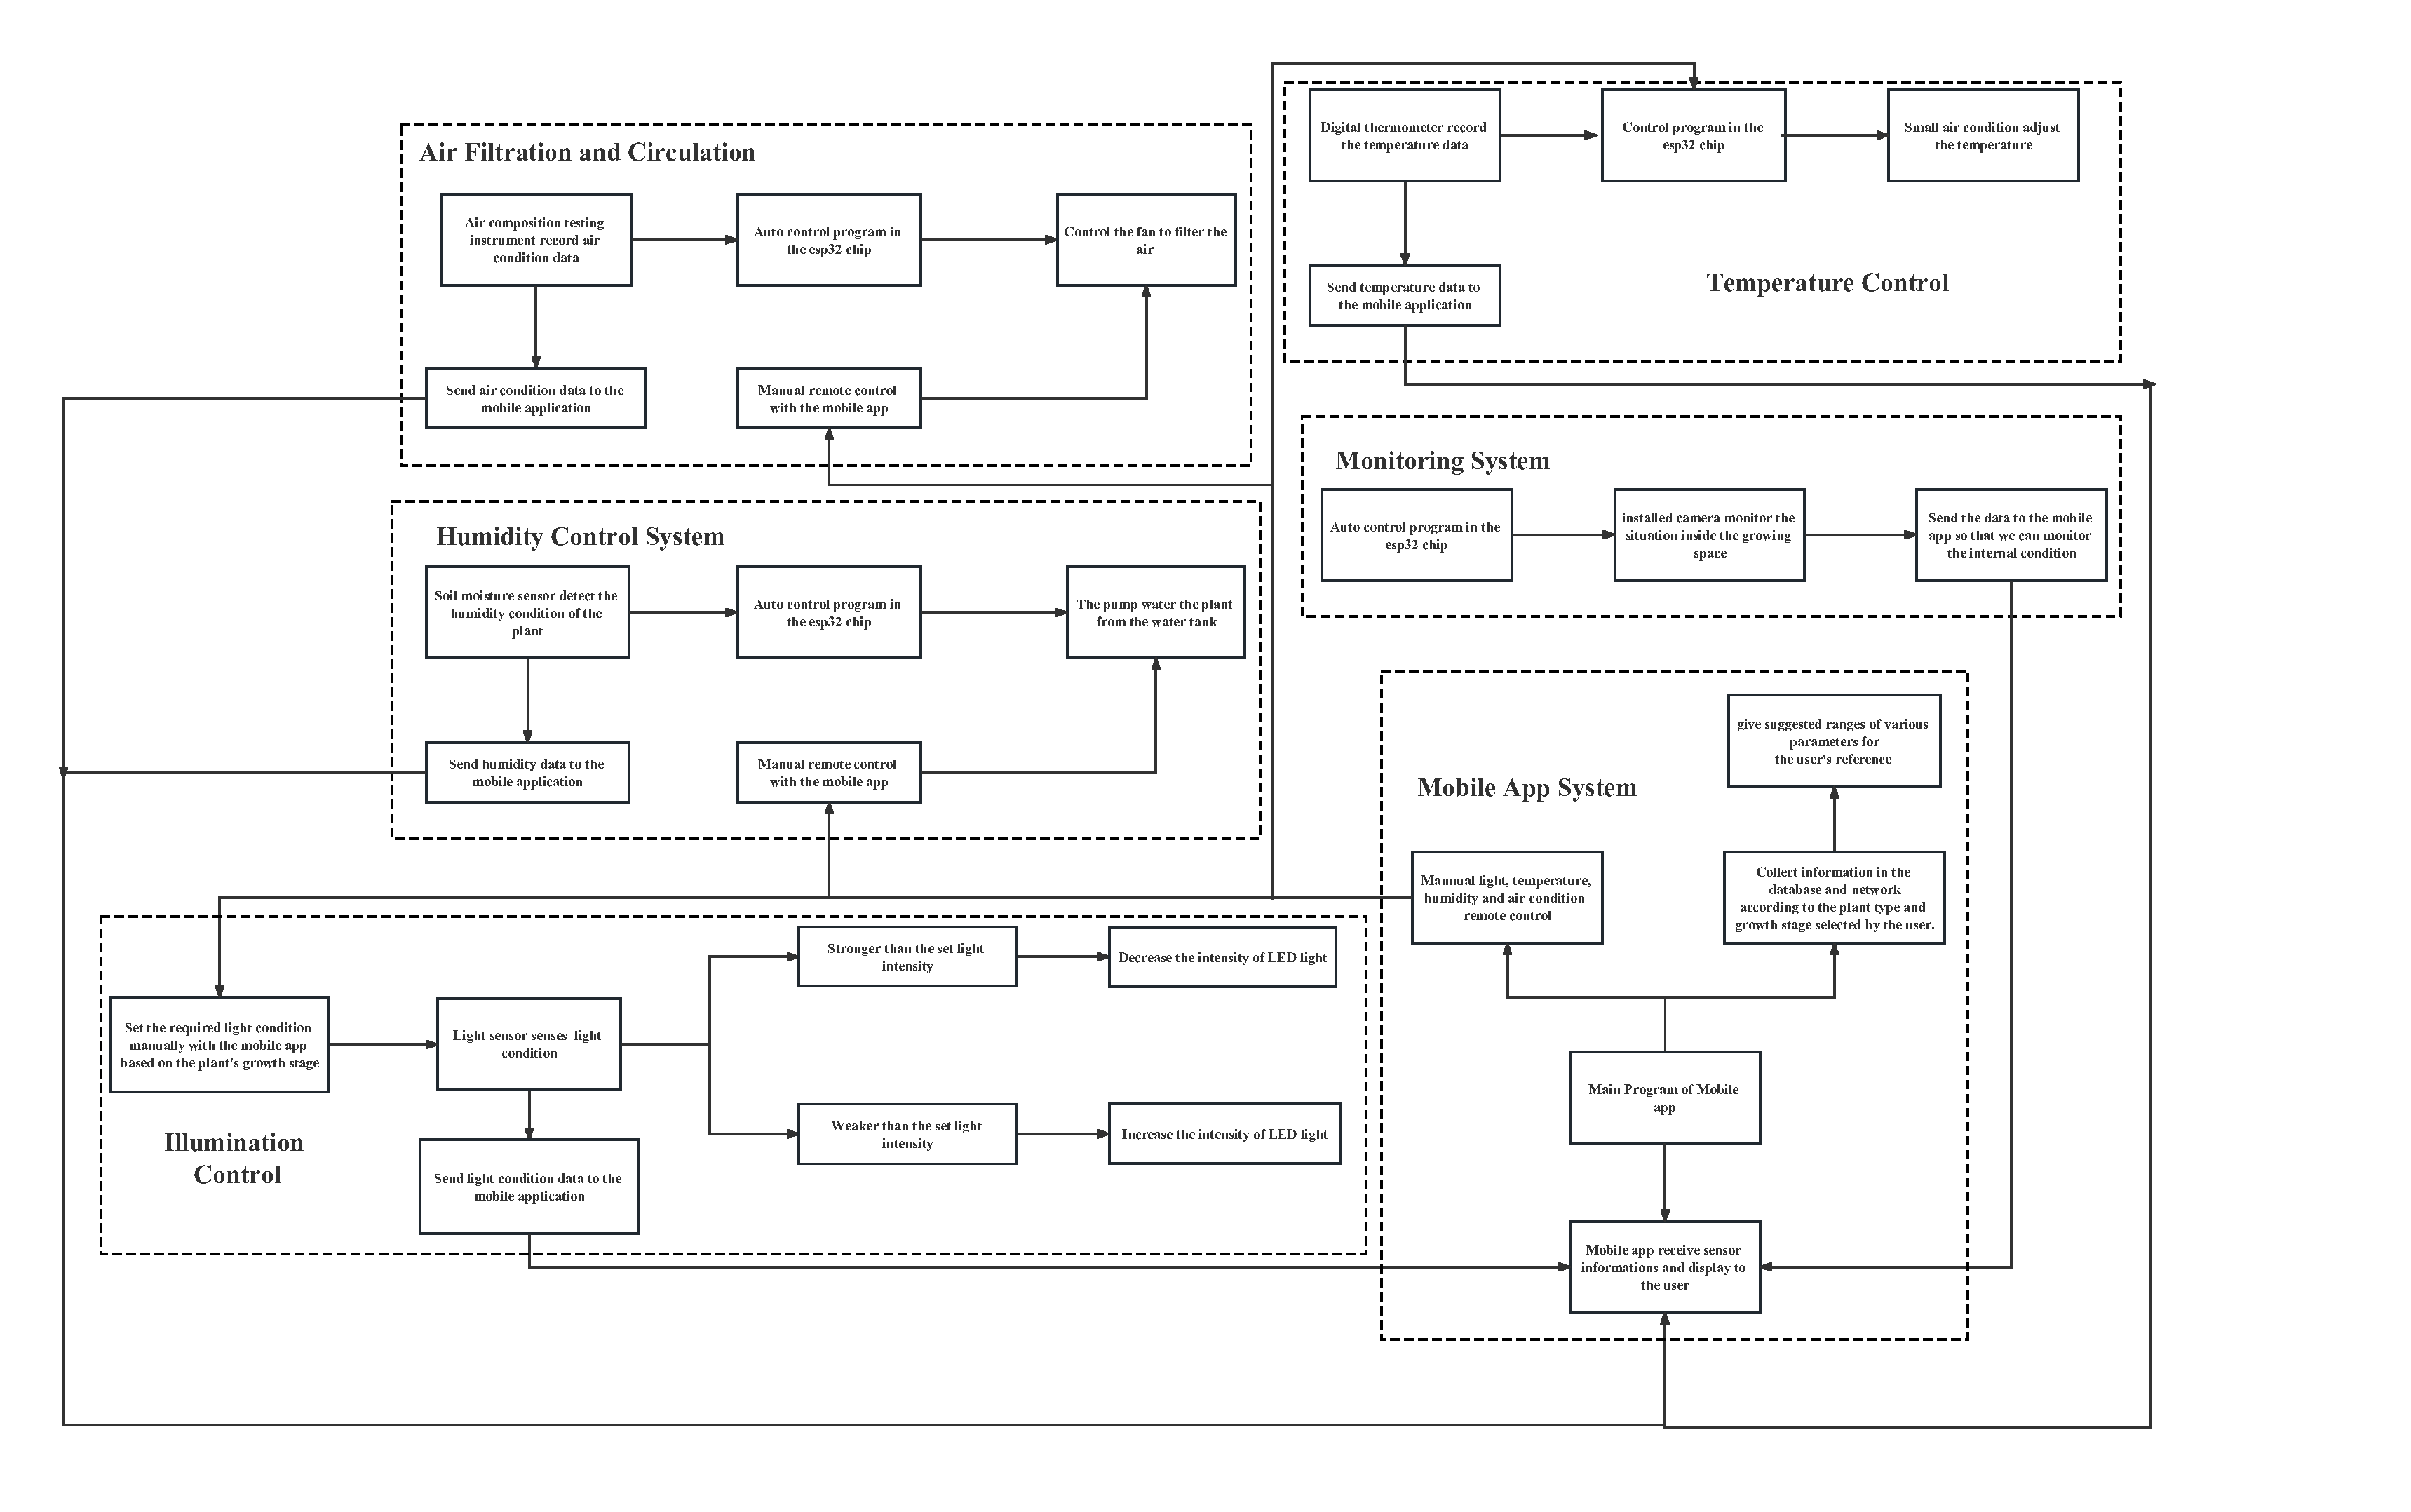
\includegraphics[width=0.8\textwidth]{Figure/detailed_block.pdf}
\caption{Detailed Subsystem}
\label{fig:d_block}
\end{figure}

\subsubsection{Growing Space}
This is the space where plants grow and is the central part of this tabletop greenhouse landscape. Environmental factors such as temperature, humidity, and this part need to be controlled by the program we designed. This desktop landscape facility is soil cultivation, and it can detect whether various environmental conditions are suitable through the mobile app.

\textbf{Requirements:} 
The shell of the model should have good light transmission (plastic or glass) and should be able to achieve excellent heat preservation and moisture retention. The vent design must not affect the functionality required by the previous two points.
% For each subsystem in your block diagram, you should include a highly detailed block description. Each description must include a statement indicating how the block contributes to the overall design dictated by the high-level requirements. Any interfaces with other blocks must be defined clearly and quantitatively. Include a list of requirements where if any of these requirements were removed, the subsystem would fail to function. Good example: Power Subsystem must be able to supply at least 500mA to the rest of the system continuously at 5V +/- 0.1V.

\subsubsection{Illumination System}
The light inside the growing space is provided by side-by-side LED devices. Since plants need different light conditions at different growth stages, we need to control the wavelength, intensity, and duration of light in the growing space by changing the light of LEDs. It is worth mentioning that the light environment outside the greenhouse is also under our consideration, such as the difference between day and night light, to maintain the stability of the light environment in the growing space. These light conditions are measured by a photoresist and portable optical wavelength meter and reflected in the mobile app.

\textbf{Requirements:}
In general, plants need more blue light when growing and maturing and then need red and orange light when blooming and producing.\cite{vercelletto_2021} The LEDs should be able to provide blue light wavelength at 400-500nm, the green light spectrum from 500-600nm, red light at 600-700nm, and far-red radiation from 700-800nm, meeting the requirements for greenhouse planting.\cite{technologies_2021}
% is connected to growth and flowering and can improve the quality of certain types of plant. When used in conjunction with other grow light spectrum wavelengths, blue light can help you tightly manage growth cycles. The green light spectrum from 500-600nm is not seen to be as useful as the other wavelengths for plant grown but it is valuable for photosynthesis and research has found that green light can ‘actually promote extension growth’ and that the results it offers depend on intensity and type of crop. Then, red light at 600-700nm is one of the most efficient grow light spectrums for photosynthesis and plant biomass growth and is one of the most efficient spectrums for plant growth and energy consumption. Finally, far-red radiation from 700-800nm can promote extension growth and ‘influences the size of the leaves, the length of stems, and ultimately the height of plants.’ 


\subsubsection{Air Circulation System}
Plants need a suitable air environment to grow, which we need to provide in the growing space. We want to achieve air filtration and circulation through a filter and fan, timed to switch on and off through the app's control program. We will also install air composition testing instruments and reflect the data in real-time on the cell phone app, which can remotely control the switch of the air circulation system.

\textbf{Requirements:}
The system should be able to adjust its exhaust airflow according to the plants in the growing space and the information received from the air quality detector. Different kinds of plants have different efficiency in filtering the air quality, while their abilities on absorbing the specific harmful particles in the air are various. For example, aloe vera is a good formaldehyde absorber, which can absorb 90\% of formaldehyde contained in 1 cubic meter of air but may have lower efficiency on other particles. 


\subsubsection{Temperature Control System}
This system controls the temperature in the growing space to meet the different needs of different plants and different growth stages of plants. We achieve temperature control through a small air conditioner that works with the air circulation system to raise or lower the temperature. At the same time, the temperature in the growing space will also be measured by a digital thermometer for real-time transmission to the cell phone app.

\textbf{Requirements:}
The temperature should be able to maintain a temperature range of around 18º-24ºC (64ºF – 75ºF), as the temperatures outside of this range would normally lead to slower or halted growth and suboptimal plant quality.\cite{devops_2022}

\subsubsection{Humidity Control System}
This system is used to provide plants with the right humidity environment for growth by adjusting the supply of water. We use a Soil Moisture Sensor to detect the humidity condition of the plants. Underneath the device, we are equipped with a water tank, which can be watered regularly through the mobile app's control or manually through a moisture sensor that detects the soil moisture condition.

\textbf{Requirements:}
The humidity control system should be able to maintain humidity around 80\%, which is a relative humidity setpoint for most plants. At this level, growth rates are highest for common greenhouse plants. At higher or lower humidity levels, plant physiological processes may slow down, leading to slower growth and lower quality output.\cite{devops_2022}

\subsubsection{Real-time Monitoring System}
The detection system can detect the growing space in real-time, and this is detected by the installed camera. At the same time, we can monitor the situation inside through the mobile app.

\textbf{Requirements:}
Currently, we don't have the requirements for video quality. To save energy, the default status for the camera module should be off. It should be manually controlled by the mobile phone.

\subsubsection{Main Control System (together with a chip microcontroller)}
The main control system is composed of an ESP32\cite{wikipedia_2023}, a Tencent Cloud Server, and a mobile phone app. All the sensors' information should be first sent to ESP32 to process and packaging. These data should be then pushed into the cloud server. The cloud server will set up a log for them. The mobile phone app can receive the information from the server and feed it back to the user. At the same time, we can also remotely control the light, temperature, humidity, and air condition in the device through the mobile app and can set the timer operation or threshold operation. The mobile app can also give suggested ranges of various parameters for the user's reference based on the information in the database and network according to the plant type and growth stage selected by the user.

\textbf{Requirements:}
ESP32 should be able to handle multiple sensors' information. The server should be able to store users' information and a database for planting. A backup for the sensors should also be included as a part of the database on the server. The basic features of the mobile phone app are like a remote controller. All the sensors' switchers are integrated into the app.

\subsection{Tolerance Analysis} 
For the growing area, there will be a challenge in the selection of the material for the shell. The temperature and humidity maintaining function will be mainly counted on this, as we do not hope that these systems are always on. A good heat and humidity insolation can save much energy, and decrease the burden on the power supply. However, if we use a 3D printer to print the model, we have limited choices in the material. 
Another challenge is the design of the LED array. In such a small space, it is hard to give a specific wavelength with sufficient light intensity. We also need to consider the affection of the luminousness of the shell, which can influence the performance of the LEDs.
 % Copy the above 3 lines to add another section

\clearpage

\clearpage
\section{Cost}
jjjjjjj % Copy the above 3 lines to add another section

\clearpage

\clearpage
\section{Ethics and Safety}
There are a few potential safety concerns that must be addressed during the development process. The first principle is that it must not hurt people. Traditionally, the main concern on house-use electrical products is the leaking of electricity. Considering that our product incorporates a lot of precision electronic components, while the working space is quite wet, the probability of a short circuit in the circuit is high. 

Another ethics-related problem is that since our product has a monitoring system, the data collected by the camera may include the user's privacy. These data should be carefully ciphered and saved on the server with necessary security protection. A leaking of information may lead to a serious problem. % Copy the above 3 lines to add another section

\clearpage

% \printbibliography[heading=bibintoc, title={References}]

% \begin{appendices}
%     \clearpage
%     \section{Example Appendix} \label{appendix:a}

An appendix can go here! Make sure you use the \verb|\label{appendix:a}| above so that you can reference this section in your document.
%     % copy the above two lines to add more appendices
% \end{appendices}
\bibliography{references}
\bibliographystyle{IEEEtran}

\end{document}
